\documentclass[12pt]{article}
\usepackage{setspace}  % To use linespacing
\usepackage{indentfirst} % Indents first line after sections
\usepackage{amssymb} % For \mathbb
\usepackage{enumerate} % For changing labels of enumerate
\usepackage[margin=1in]{geometry} % For editing margins
\usepackage{tikz} % Tikz drawing for graphs
\usetikzlibrary{arrows.meta} % Allows customizing arrows
\usetikzlibrary{backgrounds} % For framing a tikzpicture
\usetikzlibrary{calc, through}
\usetikzlibrary{decorations.markings}
\usetikzlibrary{arrows}
\usetikzlibrary{positioning}
\usepackage{amsmath}
\usepackage{ifthen}
\usepackage{intcalc} % \intcalcMod

% Make new commands
\newcommand{\N}{\mathbb{N}}
\newcommand{\R}{\mathbb{R}}
\newcommand{\Z}{\mathbb{Z}}
\newcommand{\abs}[1]{\left|#1\right|}
\newcommand{\paren}[1]{\left(#1\right)}
\newcommand{\fivespace}{\space\space\space\space\space}

\newcommand{\be}{\begin{enumerate}}
\newcommand{\ee}{\end{enumerate}}
\newcommand{\seti}[1]{\setcounter{enumi}{#1}}
\newcommand{\setii}[1]{\setcounter{enumii}{#1}}

% Start main document
\begin{document}
\onehalfspacing
\hfill Frank Cline

\hfill Math 307

\hfill HW 9

% PROBLEMS
\section*{Problems 1-4}

\be
% 1
\item Find a plane drawing of the following graphs. Label your graph to demonstrate the isomorphism. For the left-hand graph, can you find a plane embedding with mirror symmetry?

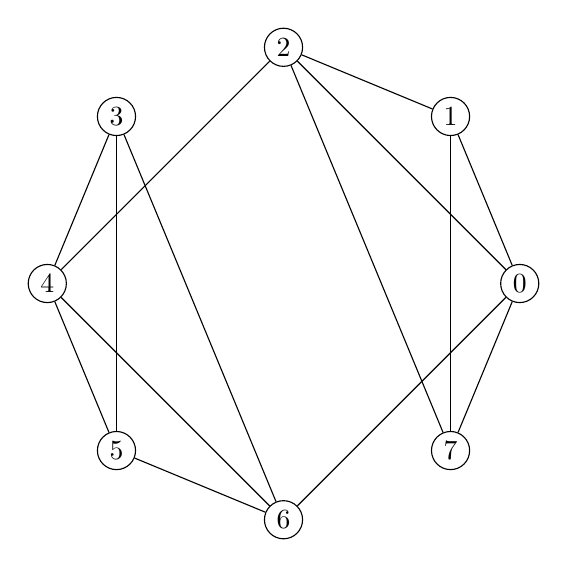
\begin{tikzpicture}
\foreach \i in {0, 1, ..., 7}{\node[draw, circle, inner sep = 2pt] (\i) at (360*\i/8: 3){\i};}
\foreach  \i/\j in {0/1, 0/2, 0/6, 0/7, 1/2, 1/7, 2/4, 2/7, 3/4, 3/5, 3/6, 4/5, 4/6, 5/6}
{\draw (\i) -- (\j);}
\end{tikzpicture}
\hspace{2cm}
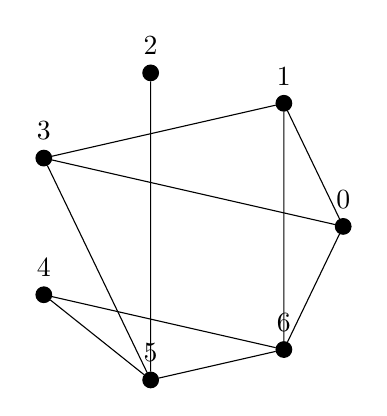
\begin{tikzpicture}[]
\foreach \i in {0, ...,6}{  \node[draw, circle, fill=black, inner sep = 2 pt, label={$\i$}](\i) at (\i*360/7: 2) {};}
\draw (1) -- (3)--(0);
\draw (2) -- (5) -- (4) -- (6) -- (0) --(1)--(6);
\draw (3) -- (5)--(6);
 \end{tikzpicture}

	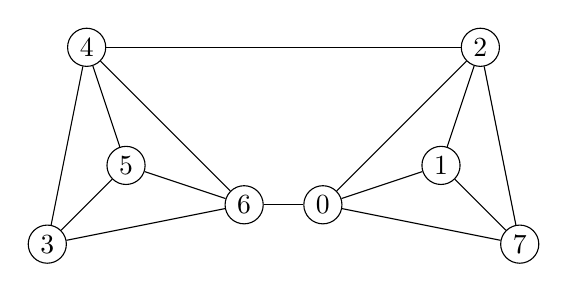
\begin{tikzpicture}
	\begin{scope}[every node/.style={circle, draw, inner sep = 2pt}]
	    	\node (2) at (3,0) {2};
		\node (1) at (2.5,-1.5) {1};
	    	\node (0) at (1,-2) {0};
		\node (7) at (3.5,-2.5) {7};
		\node (4) at (-2,0) {4};	
		\node (6) at (0,-2) {6};
		\node (3) at (-2.5,-2.5) {3};
		\node (5) at (-1.5,-1.5) {5};
	\end{scope}
	
	\begin{scope}[>={Stealth[black]},
	              every node/.style={fill=white,circle},
	              every edge/.style={draw=black}]
		\path (0) edge (1);
		\path (0) edge (2);
		\path (0) edge (6);
		\path (0) edge (7);
		\path (1) edge (7);
		\path (2) edge (1);
		\path (2) edge (4);
		\path (2) edge (7);
		\path (3) edge (4);
		\path (3) edge (5);
		\path (3) edge (6);
		\path (4) edge (5);
		\path (4) edge (6);
		\path (5) edge (6);
	\end{scope}
	\end{tikzpicture}
	\hspace{2cm}
		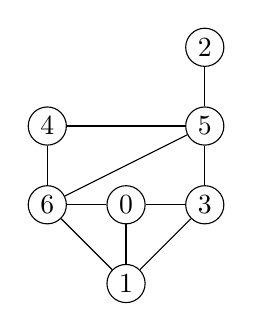
\begin{tikzpicture}
	\begin{scope}[every node/.style={circle, draw, inner sep = 2pt}]
	    	\node (0) at (0,1) {0};
		\node (1) at (0,0) {1};
	    	\node (2) at (1,3) {2};
	    	\node (3) at (1,1) {3};
	    	\node (4) at (-1,2) {4};
	    	\node (5) at (1,2) {5};
	    	\node (6) at (-1,1) {6};
	\end{scope}
	
	\begin{scope}[>={Stealth[black]},
	              every node/.style={fill=white,circle},
	              every edge/.style={draw=black}]
		\path (0) edge (1);
		\path (0) edge (3);
		\path (0) edge (6);
		\path (1) edge (3);
		\path (1) edge (6);
		\path (2) edge (5);
		\path (3) edge (5);
		\path (4) edge (5);
		\path (4) edge (6);
		\path (5) edge (6);
	\end{scope}
	\end{tikzpicture}

% 2
\item 
	\be
	% 2 a
        \item Suppose that $G$ is a triangle-free, simple, connected plane graph with at least 3 vertices. Show
         that $E\leq 2V - 4$, by counting the edges around all the faces and using Euler's Theorem.\\
       		Since $G$ is a connected plane graph, we know $V-E+F=2$. That means $F=2-V+E$.\\
		When $V=1,E=0$. $0\not\leq2(1)-4$.\\
		When $V=2,E=2$. $2\not\leq2(2)-4$	\\
		When $V=3,E\leq2$. $2\leq2(3)-4$\\
		If $V\geq3$, then
		\begin{align*}
		2E &= 4(F_4)+5(F_5)+6(F_6)+...+n(F_n)\\
		     &\geq 4(F_4)+4(F_5)+4(F_6)+...+4(F_n)\\
		     &= 4F\\
		     &= 4(2-V+E)\hspace{1cm}\text{(By Euler's Theorem)}\\
		     &= 8-4V+4E\\
		2E &\geq 8-4V+4E\\
		4V-8 &\geq 2E\\
		E &\leq 2V-4
		\end{align*}
		Thus, $E\leq 2V-4$ when $V\geq3$ and graph $G$ is a triangle-free, simple, connected plane 
		graph.
		
       	% 2 b 
        \item Use the previous result to show that $K_{3,3}$ is not planar.\\
        		$K_{3,3}$ has the properties: $V=6, E=9$, and it is also a simple, connected graph with no 
		triangle faces, so $E\leq 2V-4$ which is $9\leq 2(6)-4$ and $9\not\leq8$.
        
        % 2 c
        \item Suppose that there are three houses on a road. Each house needs to be connected to gas, 
        water, and electricity, via an underground connection. Is there a way to make all nine connections 
        without any of the lines crossing each other? (Having to dig on one plane is much cheaper than having 
        to route some of the connections below the others!) If not, what is the fewest number of crossings 
        possible?\\
       		The graph would be isomorphic to the $K_{3,3}$ graph because all each of the 3 houses 
		connects to each of the 3 services, so using the previous question, it it not possible to make all 
		nine connections without any of the lines crossing. The smallest number of crossings necessary 
		is one, as illustrated below. 
		\vspace{0.5cm}\\
		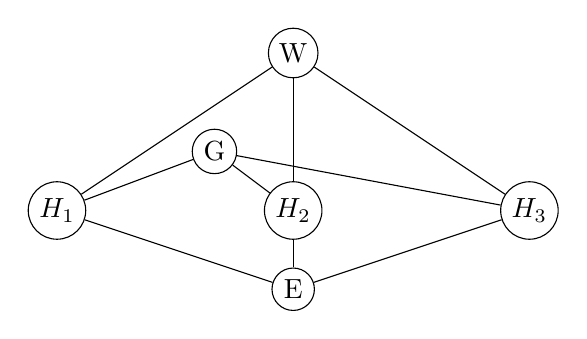
\begin{tikzpicture}
                	\begin{scope}[every node/.style={circle, draw, inner sep = 2pt}]
                	    	\node (1) at (0,0) {$H_1$};
                		\node (2) at (3,0) {$H_2$};
                	    	\node (3) at (6,0) {$H_3$};
                		\node (E) at (3,-1) {E};
                		\node (W) at (3,2) {W};	
                		\node (G) at (2,0.75) {G};
                	\end{scope}
                	
                	\begin{scope}[>={Stealth[black]},
                	              every node/.style={fill=white,circle},
                	              every edge/.style={draw=black}]
                		\foreach \i in {1,2,3}  
			{
				\path (\i) edge (E);
				\path (\i) edge (W);
				\path (\i) edge (G);
			}
                	\end{scope}
                	\end{tikzpicture}
        \ee
        
% 3
\item 
        \be 
       % 3 a
        \item Suppose that $G$ is a connected simple plane graph, where every vertex is degree 3, that 
        only has pentagons and hexagons as faces. Show that $G$ must have exactly 12 pentagons.\\
        Let $F_5\text{ and }F_6$ be the number of faces that are pentagons and hexagons. We know:
        		\begin{align*}
        		2E&=5(F_5) + 6(F_6) =\text{sum of deg(v) for } v\in(V(G)) = 3V\\
		E &= \frac{5}{2}(F_5) + 3(F_6)\\
		V &= \frac{5}{3}(F_5) + 2(F_6)\\
		F &= F_5 + F_6\\
		2 &= V-E+F \\
		&= \paren{\frac{5}{3}(F_5) + 2(F_6)} - \paren{\frac{5}{2}(F_5) + 3(F_6)} + \paren{F_5 + F_6}
		= \frac{1}{6}(F_5)\\
		2(6) &= 12 = F_5
		\end{align*}
        		Thus, we know there must be exactly 12 faces that are pentagons.
        % 3 b
        \item In the above situation, what is the smallest graph $G$ with this property? (Hint: what's the fewest 
        number of hexagons possible in such a situation?)\\
        		The smallest graph would be a graph with no hexagons, so $F_6=0$.
        		\begin{align*}
		2E &= 3V = 5(F_5) + 6(F_6) \\
		2E &= 3V = 5(12) = 60 \\
		F &= F_5 + F_6 = 12 + 0 = 12\\
		E &= 60\div2 = 30 \\
		V &= 60\div3 = 20 
		\end{align*}
		Thus the smallest graph $G$ has 20 vertices, 30 edges, and 12 faces.
        \ee
        
% 4        
\item Go find out about a planarity testing algorithm and describe how it works.\\
	The algorithm I found is the Hopcroft algorithm. The way it works is a tree is produced from a Depth 
	First Search. It uses the edges in the DFS that form a cycle and then it uses the subgraphs that 
	connect to the cycle. Each subgraph is then tested for planarity, and if it is plane, the plane drawing is 
	added to the plane graph. This continues until the entire graph has been added to the plane drawing.

\ee

\end{document}















